%  LaTeX support: latex@mdpi.com
%  For support, please attach all files needed for compiling as well as the log file, and specify your operating system, LaTeX version, and LaTeX editor.

%=================================================================
% pandoc conditionals added to preserve backwards compatibility with previous versions of rticles

\documentclass[notspecified,article,submit,moreauthors,pdftex]{Definitions/mdpi}


%% Some pieces required from the pandoc template
\setlist[itemize]{leftmargin=*,labelsep=5.8mm}
\setlist[enumerate]{leftmargin=*,labelsep=4.9mm}


%--------------------
% Class Options:
%--------------------

%---------
% article
%---------
% The default type of manuscript is "article", but can be replaced by:
% abstract, addendum, article, book, bookreview, briefreport, casereport, comment, commentary, communication, conferenceproceedings, correction, conferencereport, entry, expressionofconcern, extendedabstract, datadescriptor, editorial, essay, erratum, hypothesis, interestingimage, obituary, opinion, projectreport, reply, retraction, review, perspective, protocol, shortnote, studyprotocol, systematicreview, supfile, technicalnote, viewpoint, guidelines, registeredreport, tutorial
% supfile = supplementary materials

%----------
% submit
%----------
% The class option "submit" will be changed to "accept" by the Editorial Office when the paper is accepted. This will only make changes to the frontpage (e.g., the logo of the journal will get visible), the headings, and the copyright information. Also, line numbering will be removed. Journal info and pagination for accepted papers will also be assigned by the Editorial Office.

%------------------
% moreauthors
%------------------
% If there is only one author the class option oneauthor should be used. Otherwise use the class option moreauthors.

%---------
% pdftex
%---------
% The option pdftex is for use with pdfLaTeX. Remove "pdftex" for (1) compiling with LaTeX & dvi2pdf (if eps figures are used) or for (2) compiling with XeLaTeX.

%=================================================================
% MDPI internal commands - do not modify
\firstpage{1}
\makeatletter
\setcounter{page}{\@firstpage}
\makeatother
\pubvolume{1}
\issuenum{1}
\articlenumber{0}
\pubyear{2023}
\copyrightyear{2023}
%\externaleditor{Academic Editor: Firstname Lastname}
\datereceived{ }
\daterevised{ } % Comment out if no revised date
\dateaccepted{ }
\datepublished{ }
%\datecorrected{} % For corrected papers: "Corrected: XXX" date in the original paper.
%\dateretracted{} % For corrected papers: "Retracted: XXX" date in the original paper.
\hreflink{https://doi.org/} % If needed use \linebreak
%\doinum{}
%\pdfoutput=1 % Uncommented for upload to arXiv.org

%=================================================================
% Add packages and commands here. The following packages are loaded in our class file: fontenc, inputenc, calc, indentfirst, fancyhdr, graphicx, epstopdf, lastpage, ifthen, float, amsmath, amssymb, lineno, setspace, enumitem, mathpazo, booktabs, titlesec, etoolbox, tabto, xcolor, colortbl, soul, multirow, microtype, tikz, totcount, changepage, attrib, upgreek, array, tabularx, pbox, ragged2e, tocloft, marginnote, marginfix, enotez, amsthm, natbib, hyperref, cleveref, scrextend, url, geometry, newfloat, caption, draftwatermark, seqsplit
% cleveref: load \crefname definitions after \begin{document}

%=================================================================
% Please use the following mathematics environments: Theorem, Lemma, Corollary, Proposition, Characterization, Property, Problem, Example, ExamplesandDefinitions, Hypothesis, Remark, Definition, Notation, Assumption
%% For proofs, please use the proof environment (the amsthm package is loaded by the MDPI class).

%=================================================================
% Full title of the paper (Capitalized)
\Title{Full title of the paper (Capitalized)}

% MDPI internal command: Title for citation in the left column
\TitleCitation{Full title of the paper (Capitalized)}

% Author Orchid ID: enter ID or remove command
%\newcommand{\orcidauthorA}{0000-0000-0000-000X} % Add \orcidA{} behind the author's name
%\newcommand{\orcidauthorB}{0000-0000-0000-000X} % Add \orcidB{} behind the author's name


% Authors, for the paper (add full first names)
\Author{Dominik
Leutnant$^{1,2,\ddagger,*}$\href{https://orcid.org/0000-0003-3293-2315}
{\orcidicon}, John Doe$^{2, \dagger, \ddagger}$}


%\longauthorlist{yes}


% MDPI internal command: Authors, for metadata in PDF
\AuthorNames{Dominik Leutnant, John Doe}

% MDPI internal command: Authors, for citation in the left column
%\AuthorCitation{Lastname, F.; Lastname, F.; Lastname, F.}
% If this is a Chicago style journal: Lastname, Firstname, Firstname Lastname, and Firstname Lastname.
\AuthorCitation{Leutnant, D.; Doe, J.}

% Affiliations / Addresses (Add [1] after \address if there is only one affiliation.)
\address{%
$^{1}$ \quad Muenster University of Applied Sciences - Institute for
Infrastructure, Water, Resources, Environment Correnstr. 25, 48149
Muenster,
Germany; \href{mailto:leutnant@fh-muenster.de}{\nolinkurl{leutnant@fh-muenster.de}}\\
$^{2}$ \quad Your department Street, City,
Country; \href{mailto:mail@mail.com}{\nolinkurl{mail@mail.com}}\\
}

% Contact information of the corresponding author
\corres{Correspondence: \href{mailto:leutnant@fh-muenster.de}{\nolinkurl{leutnant@fh-muenster.de}};
Tel.: +XX-000-00-0000.}

% Current address and/or shared authorship
\firstnote{Current address: Updated affiliation}
\secondnote{These authors contributed equally to this work.}






% The commands \thirdnote{} till \eighthnote{} are available for further notes

% Simple summary
\simplesumm{A Simple summary goes here.}

%\conference{} % An extended version of a conference paper

% Abstract (Do not insert blank lines, i.e. \\)
\abstract{A single paragraph of about 200 words maximum. For research
articles, abstracts should give a pertinent overview of the work. We
strongly encourage authors to use the following style of structured
abstracts, but without headings: 1) Background: Place the question
addressed in a broad context and highlight the purpose of the study; 2)
Methods: Describe briefly the main methods or treatments applied; 3)
Results: Summarize the article's main findings; and 4) Conclusion:
Indicate the main conclusions or interpretations. The abstract should be
an objective representation of the article, it must not contain results
which are not presented and substantiated in the main text and should
not exaggerate the main conclusions.}


% Keywords
\keyword{keyword 1; keyword 2; keyword 3 (list three to ten pertinent
keywords specific to the article, yet reasonably common within the
subject discipline.).}

% The fields PACS, MSC, and JEL may be left empty or commented out if not applicable
%\PACS{J0101}
%\MSC{}
%\JEL{}

%%%%%%%%%%%%%%%%%%%%%%%%%%%%%%%%%%%%%%%%%%
% Only for the journal Diversity
%\LSID{\url{http://}}

%%%%%%%%%%%%%%%%%%%%%%%%%%%%%%%%%%%%%%%%%%
% Only for the journal Applied Sciences

%%%%%%%%%%%%%%%%%%%%%%%%%%%%%%%%%%%%%%%%%%

%%%%%%%%%%%%%%%%%%%%%%%%%%%%%%%%%%%%%%%%%%
% Only for the journal Data



%%%%%%%%%%%%%%%%%%%%%%%%%%%%%%%%%%%%%%%%%%
% Only for the journal Toxins


%%%%%%%%%%%%%%%%%%%%%%%%%%%%%%%%%%%%%%%%%%
% Only for the journal Encyclopedia


%%%%%%%%%%%%%%%%%%%%%%%%%%%%%%%%%%%%%%%%%%
% Only for the journal Advances in Respiratory Medicine
%\addhighlights{yes}
%\renewcommand{\addhighlights}{%

%\noindent This is an obligatory section in “Advances in Respiratory Medicine”, whose goal is to increase the discoverability and readability of the article via search engines and other scholars. Highlights should not be a copy of the abstract, but a simple text allowing the reader to quickly and simplified find out what the article is about and what can be cited from it. Each of these parts should be devoted up to 2~bullet points.\vspace{3pt}\\
%\textbf{What are the main findings?}
% \begin{itemize}[labelsep=2.5mm,topsep=-3pt]
% \item First bullet.
% \item Second bullet.
% \end{itemize}\vspace{3pt}
%\textbf{What is the implication of the main finding?}
% \begin{itemize}[labelsep=2.5mm,topsep=-3pt]
% \item First bullet.
% \item Second bullet.
% \end{itemize}
%}


%%%%%%%%%%%%%%%%%%%%%%%%%%%%%%%%%%%%%%%%%%


% tightlist command for lists without linebreak
\providecommand{\tightlist}{%
  \setlength{\itemsep}{0pt}\setlength{\parskip}{0pt}}



\usepackage{longtable}

\begin{document}



%%%%%%%%%%%%%%%%%%%%%%%%%%%%%%%%%%%%%%%%%%

\begin{table}

\caption{\label{tab:mdpitype}MDPI article types.}
\centering
\begin{tabular}[t]{lll}
\toprule
abstract & entry & retraction\\
addendum & expressionofconcern & review\\
article & extendedabstract & perspective\\
book & datadescriptor & protocol\\
bookreview & editorial & shortnote\\
\addlinespace
briefreport & essay & studyprotocol\\
casereport & erratum & systematicreview\\
comment & hypothesis & supfile\\
commentary & interestingimage & technicalnote\\
communication & obituary & viewpoint\\
\addlinespace
conferenceproceedings & opinion & guidelines\\
correction & projectreport & registeredreport\\
conferencereport & reply & tutorial\\
\bottomrule
\end{tabular}
\end{table}

\section{Introduction}\label{introduction}

\subsection{POMDP}\label{pomdp}

\subsection{Simulation details}\label{simulation-details}

The simulated enviroment features discretized of planning cancer
treatments. At each timestep a ``cancer state'' has a certain risk of
increasing. If the tumor ever reaches the state 5, the simulation ends.
To avoid this, a model has decide when to apply treatment. Applying
treatment can reduce the tumor level - whether the treatment succesfully
reduces the ``cancer state'' depends on a underlying \emph{resistance
state}. When the resistance is low, the chance of treatment succeeding
is high, but probability declines as the resistance state increase. The
resistance state has fixed probability of increasing when treatment is
applied, and it can decrease when treatment is withdrawn. Whether the
resistance state decreases depends on the tumor level. At high tumor
levels, the resistance state is more likely to decrease, but thiscarries
the risk of tumor growing out of control and ``killing the patient''. In
order to succesfully manage the disease, a model will therefore also
have to manage the resistance state. However, the resistance state is
directly orbserable in the given simulation. It must therefore be
inferred from how the tumor state responds to treatment.

Both the resistance state, and tumor states start at state 0 out of 5,
meaning that a total is six states are possible in each. Two slightly
different simulations are used:

\begin{itemize}
\item
  Performance simulation, where a range-bounded approach to managing the
  tumor is used, where the treatment is begun each time the tumor state
  increases above level 3, and is withdrawn when the tumor state drops
  below 2. 100 runs at 4 different probabilities of increasing the tumor
  state is run for maximally 200 timesteps. For each run, vectors of
  outcomes are pregenerated, meaning that vector of whether the tumor
  increases of length 200 is predetermined where each entry has the
  probability specified for the entire simulation. Likewise vectors are
  generated for treatment outcomes at each resistance level, and
  outcomes for resistance drops. This is done to ensure comparibility
  between the range-bounded approach and POMDP models that consider
  different future outcomes at different lengths. In these runs the
  tumor state is perfectly observable, meaning a tumor state always
  generates tumor observation that corresponds to hidden factor. The
  POMPD can only observe the tumor level, and its prior preferences are
  uniform over all tumor states except for the highest. These POMPDS
  only consider a combination of policies at each timestep. They can
  only consider treating or not treating for three timesteps in a row.
  The shortest horizon model only considers one of these blocks, while
  the medium considers two blocks of treating or not treating, for total
  horizon of 6 steps into the future. The longest horizon model
  considers three blocks for a total of 9 steps into the future. This is
  done to ease the computational burden, since it greatly reduces the
  total number of policies to be evaluated.
\item
  In the capacities simulation, a single run of a POMDP with a slightly
  different model structure is used. This model can observes a perfect
  signal of whether the patients is alive, whether the model is testing,
  treating and a noised signal of the tumor state if the model has
  decided to test the patient on the given run. Its prior preferences
  are heavily skewed against observing a dead patient, somewhat against
  treating and little against treating. This means that it will have to
  balance the ``cost'' of all these actions''. It is also handicapped
  further by the fact that the tumor signal is noised, and the
  resistance state, which must be inferred through the tumor signal is
  therefore doubly obfuscated.
\end{itemize}

\section{Results}\label{results}

\subsection{Performance of POMDPs vs ADT
heuristic}\label{performance-of-pomdps-vs-adt-heuristic}

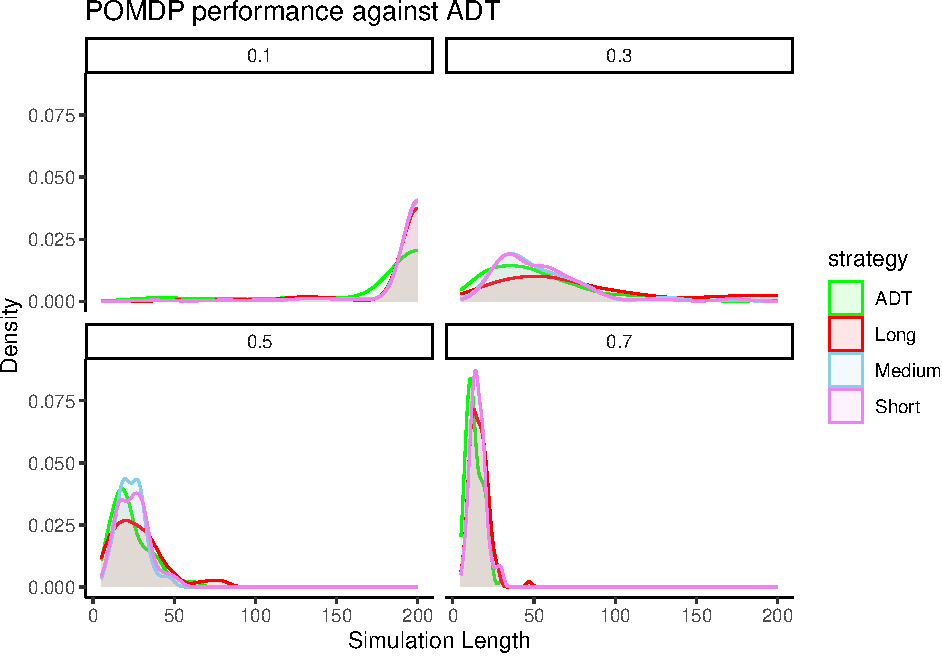
\includegraphics{SocultPaper_files/figure-latex/unnamed-chunk-1-1.pdf}

Four different simulation runs each consisting of 100 runs, of maximally
200 timesteps for different rates of tumor growth (respectively 1. .3,
.5, and .7 probability of increasing the tumor state) . On each run the
the outcomes on each of the potential 200 random variables are generated
and each strategy is therefore tested on a the same enviroment. On the
lowest tumor growth rate almost all the runs reach maximal length.

Contrasts against ADT-performance for growth rate .3, .5 and .7 are
plotted. .1 is omitted since it appears that maximal perforamnce was
achieved for each policy horizon of the POMPD strategies.

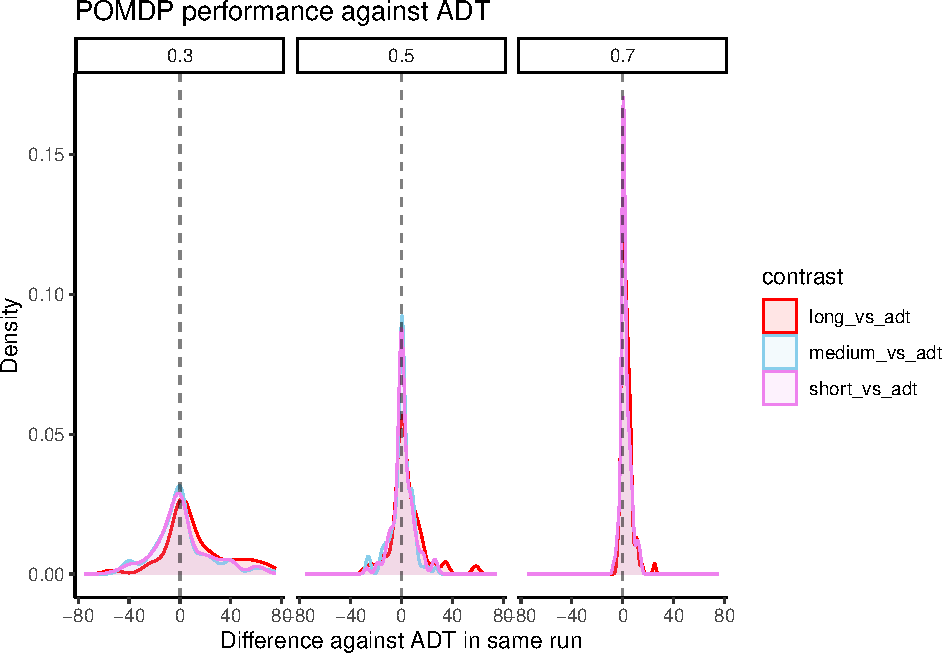
\includegraphics{SocultPaper_files/figure-latex/unnamed-chunk-2-1.pdf}

Two interpretations emerge from the contrasted simulation lengths. As
the the growth rate increases, the POMDP seems to run for longer than
the specific instance of the range bounded approach. It also seems that
longer policy horizon seems beneficial. When the tumor state had .7
probability of increasing each timestep, the longest POMPD with the
longest policy horizon performed as follows.

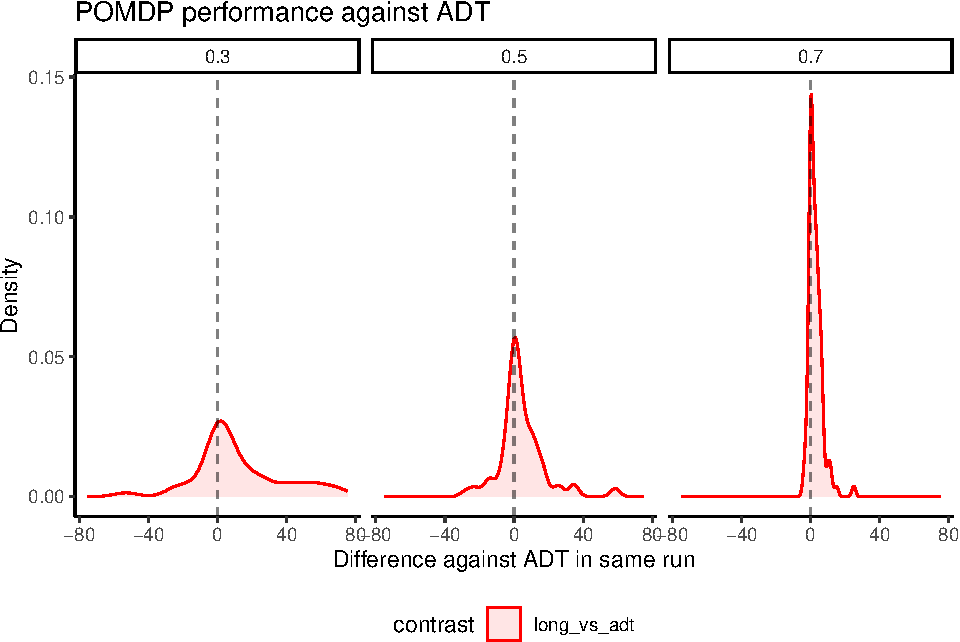
\includegraphics{SocultPaper_files/figure-latex/unnamed-chunk-3-1.pdf}

At more aggressive cancer rates, the simulation consistently to
outperform the range bounded approach. The absoulute increase in
timesteps decreases however.

\subsection{Capabilities}\label{capabilities}

\subsubsection{Learning underlying hidden
state}\label{learning-underlying-hidden-state}

The POMDP structure is capable of inferring an underlying hidden state:
the resistance state. Even though this not directly observable, this can
be inferred to how the tumor state responds to treatment. Applying
treatment for longer time without any beneficial effect would suggest
that the resistance level is high, while immediately observing that the
tumor level decreases would suggest that the resistance level is low. At
each timestep the POMDPs perform infer the most likely state of every
state factor, given their current observation and prior beliefs. Through
custom changes to the `get\_expected\_states' function in PYMDP that
allowed the models to consider how one hidden state factor (resistance
factor) would influence another (the tumor factor).

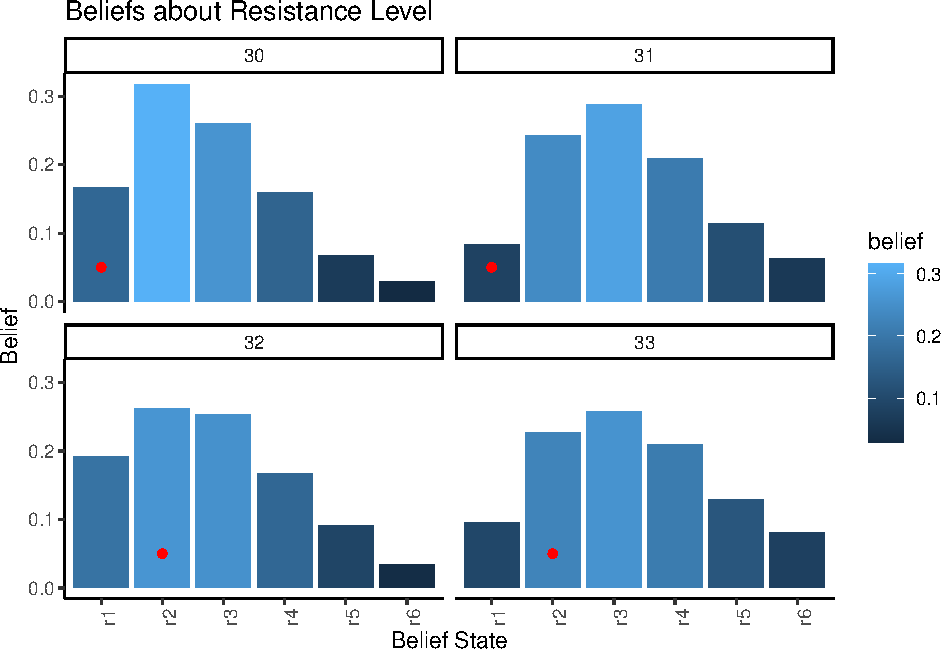
\includegraphics{SocultPaper_files/figure-latex/unnamed-chunk-4-1.pdf}

The above plot shows the strength of beliefs in t probabilities for a
subset of timesteps {[}30 - 34{]}, and the red dot show the actual the
resistance levels. A time progresses the resistance level increases, and
the model adjusts its beliefs. While the tumor level doesn't increase
durings this time\_period, this would also signal the model that the
resistance level is low. This is the case since the enviroment always
has change of increasing the tumor state, but such an increase would be
negated by succesful round of treatment.

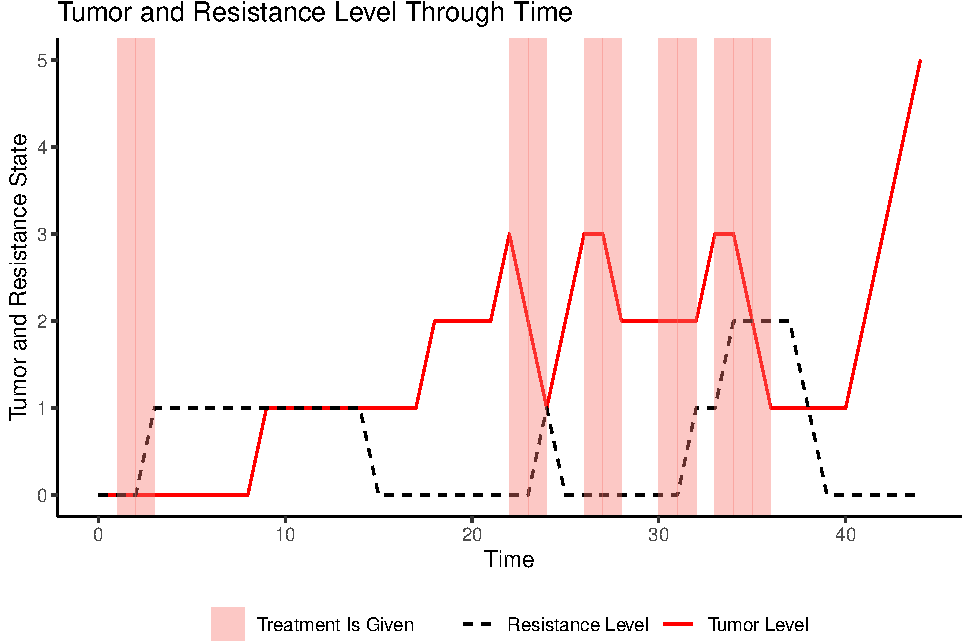
\includegraphics{SocultPaper_files/figure-latex/unnamed-chunk-5-1.pdf}

The entire run is plotted for the given. Only the tumor level is
observable to the POMDP. It must combine its knowledge about how
resistance level likely increases after applying treatment, and how the
tumor level responds to treatment depenping on the the resistance level.
While the model far from perfectly knows the resistance level. Model
beliefs for the entire run is plotted.

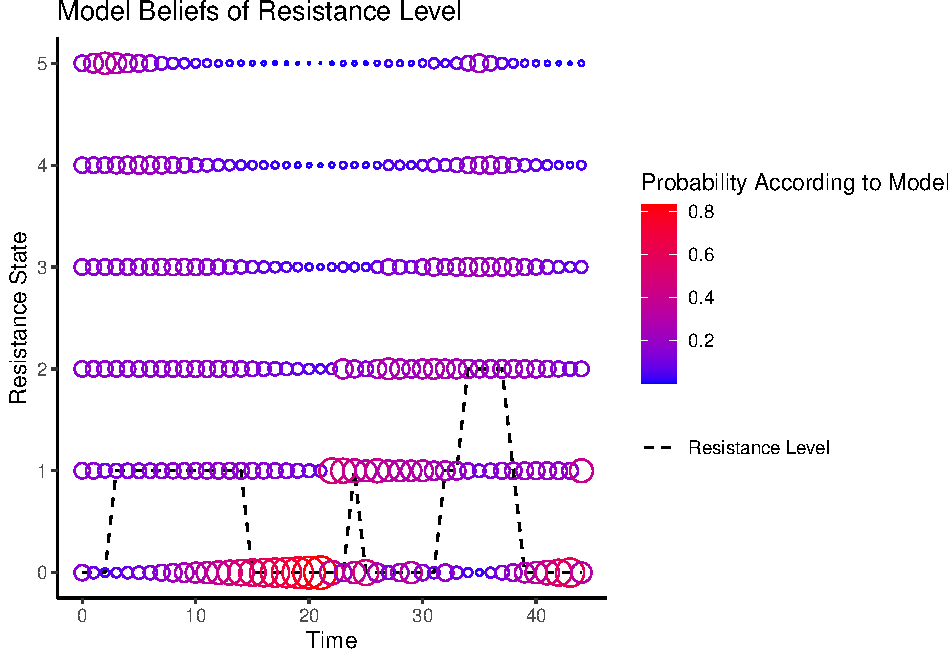
\includegraphics{SocultPaper_files/figure-latex/unnamed-chunk-6-1.pdf}

The model begins fairly agnostic. Given that the model was initialized
with a uniform prior over resistance states this makes sense. Thorought
out the course of the simulation it then finds loweer values of
resistance state more likely.

\subsubsection{Beliefs, current/future and uncertainty is
accessible}\label{beliefs-currentfuture-and-uncertainty-is-accessible}

This current simulated model used a slightly different implementation
than those compared to performance of rangebounded therapy planning.
While the those models had longer policy horizons, they didn't consider
the entire space possible actions. A model with a shorter policy horizon
that would instead search every single possible action four steps is
plotted to investigate the structure of decision-making by the POMDP
model. The enviroment was also more unceartain. Instead of featuring a
1-to-1 mapping of the observations of the tumor to actual tumor state,
it recieved a noised signal. It must therefore. The beliefs about how
tumor state will evolve as a consequence of the most promising policy at
time step 14 is plotted, and the expectation of resistance states at
t=24 is plotted too.

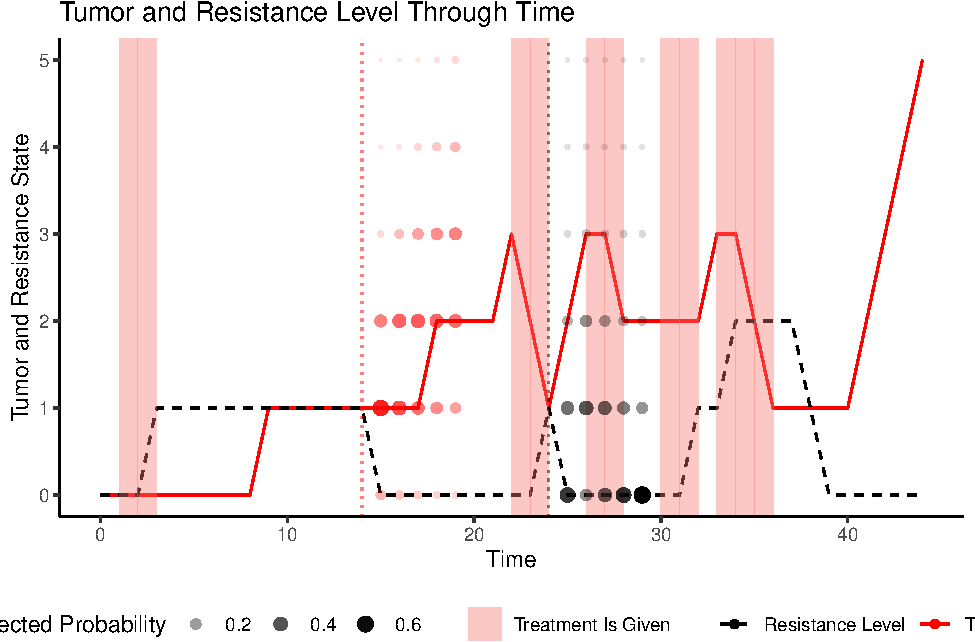
\includegraphics{SocultPaper_files/figure-latex/unnamed-chunk-7-1.pdf}

Dotted vertical lines indicated the timepoint for which the evaluation
of exepected states are extracted.

\subsubsection{Actions Can be balanced using
FEP}\label{actions-can-be-balanced-using-fep}

\subsubsection{FEP components are
accesible}\label{fep-components-are-accesible}

\section{Discussion}\label{discussion}

\subsection{Does it work for other sorts of medical
planning}\label{does-it-work-for-other-sorts-of-medical-planning}

\subsection{Would longer policy search be
better}\label{would-longer-policy-search-be-better}

\subsection{Only one range bound}\label{only-one-range-bound}

\subsection{Future Research}\label{future-research}

\subsubsection{Continuous state space or binning
illness}\label{continuous-state-space-or-binning-illness}

\subsubsection{Learning the transition
parameters}\label{learning-the-transition-parameters}

\subsubsection{searching policy space
better}\label{searching-policy-space-better}

\subsubsection{other fep models}\label{other-fep-models}

%%%%%%%%%%%%%%%%%%%%%%%%%%%%%%%%%%%%%%%%%%

\vspace{6pt}

%%%%%%%%%%%%%%%%%%%%%%%%%%%%%%%%%%%%%%%%%%
%% optional
\supplementary{The following supporting information can be downloaded
at:\\
\linksupplementary{s1}, Figure S1: title; Table S1: title; Video S1:
title.}

% Only for the journal Methods and Protocols:
% If you wish to submit a video article, please do so with any other supplementary material.
% \supplementary{The following supporting information can be downloaded at: \linksupplementary{s1}, Figure S1: title; Table S1: title; Video S1: title. A supporting video article is available at doi: link.}

%%%%%%%%%%%%%%%%%%%%%%%%%%%%%%%%%%%%%%%%%%
\authorcontributions{For research articles with several authors, a short
paragraph specifying their individual contributions must be provided.
The following statements should be used ``X.X. and Y.Y. conceive and
designed the experiments; X.X. performed the experiments; X.X. and Y.Y.
analyzed the data; W.W. contributed reagents/materials/analysis tools;
Y.Y. wrote the paper.'\,' Authorship must be limited to those who have
contributed substantially to the work reported.}

\funding{Please add:
\texttt{This\ research\ received\ no\ external\ funding\textquotesingle{}\textquotesingle{}\ or}This
research was funded by NAME OF FUNDER grant number XXX.'\,' and and
``The APC was funded by XXX'\,'. Check carefully that the details given
are accurate and use the standard spelling of funding agency names at
\url{https://search.crossref.org/funding}, any errors may affect your
future funding.}

\institutionalreview{In this section, you should add the Institutional
Review Board Statement and approval number, if relevant to your study.
You might choose to exclude this statement if the study did not require
ethical approval. Please note that the Editorial Office might ask you
for further information. Please add ``The study was conducted in
accordance with the Declaration of Helsinki, and approved by the
Institutional Review Board (or Ethics Committee) of NAME OF INSTITUTE
(protocol code XXX and date of approval).'' for studies involving
humans. OR ``The animal study protocol was approved by the Institutional
Review Board (or Ethics Committee) of NAME OF INSTITUTE (protocol code
XXX and date of approval).'' for studies involving animals. OR ``Ethical
review and approval were waived for this study due to REASON (please
provide a detailed justification).'' OR ``Not applicable'' for studies
not involving humans or animals.}

\informedconsent{Any research article describing a study involving
humans should contain this statement. Please add
\texttt{Informed\ consent\ was\ obtained\ from\ all\ subjects\ \ involved\ in\ the\ study.\textquotesingle{}\textquotesingle{}\ OR}Patient
consent was waived due to REASON (please provide a detailed
justification).'\,' OR ``Not applicable'\,' for studies not involving
humans. You might also choose to exclude this statement if the study did
not involve humans.

Written informed consent for publication must be obtained from
participating patients who can be identified (including by the patients
themselves). Please state ``Written informed consent has been obtained
from the patient(s) to publish this paper'\,' if applicable.}

\dataavailability{We encourage all authors of articles published in MDPI
journals to share their research data. In this section, please provide
details regarding where data supporting reported results can be found,
including links to publicly archived datasets analyzed or generated
during the study. Where no new data were created, or where data is
unavailable due to privacy or ethical re-strictions, a statement is
still required. Suggested Data Availability Statements are available in
section ``MDPI Research Data Policies'' at
\url{https://www.mdpi.com/ethics}.}

\acknowledgments{All sources of funding of the study should be
disclosed. Please clearly indicate grants that you have received in
support of your research work. Clearly state if you received funds for
covering the costs to publish in open access.}

\conflictsofinterest{Declare conflicts of interest or state `The authors
declare no conflict of interest.' Authors must identify and declare any
personal circumstances or interest that may be perceived as
inappropriately influencing the representation or interpretation of
reported research results. Any role of the funding sponsors in the
design of the study; in the collection, analyses or interpretation of
data in the writing of the manuscript, or in the decision to publish the
results must be declared in this section. If there is no role, please
state `The founding sponsors had no role in the design of the study; in
the collection, analyses, or interpretation of data; in the writing of
the manuscript, an in the decision to publish the results'.}

%%%%%%%%%%%%%%%%%%%%%%%%%%%%%%%%%%%%%%%%%%
%% Optional
\sampleavailability{Samples of the compounds \ldots\ldots{} are
available from the authors.}

%% Only for journal Encyclopedia

\abbreviations{Abbreviations}{
The following abbreviations are used in this manuscript:\\

\noindent
\begin{tabular}{@{}ll}
MDPI & Multidisciplinary Digital Publishing Institute \\
DOAJ & Directory of open access journals \\
TLA & Three letter acronym \\
LD & linear dichroism \\
\end{tabular}}

%%%%%%%%%%%%%%%%%%%%%%%%%%%%%%%%%%%%%%%%%%
%% Optional
\input{"appendix.tex"}
%%%%%%%%%%%%%%%%%%%%%%%%%%%%%%%%%%%%%%%%%%
\begin{adjustwidth}{-\extralength}{0cm}

%\printendnotes[custom] % Un-comment to print a list of endnotes


\reftitle{References}
\bibliography{mybibfile.bib}

% If authors have biography, please use the format below
%\section*{Short Biography of Authors}
%\bio
%{\raisebox{-0.35cm}{\includegraphics[width=3.5cm,height=5.3cm,clip,keepaspectratio]{Definitions/author1.pdf}}}
%{\textbf{Firstname Lastname} Biography of first author}
%
%\bio
%{\raisebox{-0.35cm}{\includegraphics[width=3.5cm,height=5.3cm,clip,keepaspectratio]{Definitions/author2.jpg}}}
%{\textbf{Firstname Lastname} Biography of second author}

%%%%%%%%%%%%%%%%%%%%%%%%%%%%%%%%%%%%%%%%%%
%% for journal Sci
%\reviewreports{\\
%Reviewer 1 comments and authors’ response\\
%Reviewer 2 comments and authors’ response\\
%Reviewer 3 comments and authors’ response
%}
%%%%%%%%%%%%%%%%%%%%%%%%%%%%%%%%%%%%%%%%%%
\PublishersNote{}
\end{adjustwidth}


\end{document}
